\section{Основные определения}
\begin{definition}
Пусть $\displaystyle T$ -- произвольное множество. Тогда набор случайных величин $\displaystyle X=( X_{t} ,\ t\in T)$, заданных на одном вероятностном пространстве $\displaystyle ( \Omega ,\ \mathcal{F} ,\ P)$, называеется \textit{случайной функцией} на $\displaystyle T$.
\end{definition}
\begin{note}
Формально не требуется, чтобы все $\displaystyle X_{t}$ принимали значения в одном пространстве.
\end{note}
\begin{note}
Множество $\displaystyle T$ чаще всего интерпретируется как "время".
\end{note}
\begin{note}
На $\displaystyle X$ можно смотреть как на функцию двух переменных, то есть $\displaystyle X=X( t,\ \omega ) ,\ \omega \in \Omega $.
\end{note}
\begin{definition}
\textit{Траекторией} (\textit{реализацией}) случайной функции $\displaystyle X=( X_{t} ,\ t\in T)$ называется функция на $\displaystyle T$ вида $\displaystyle \tilde{X}_{\omega _{0}}( t) =X_{t}( \omega _{0}) ,\ \omega _{0} \in \Omega ,\ t\in T$.
\end{definition}
\begin{definition}
Если $\displaystyle T\subseteq \mathbb{R}$, то случайная функция на $\displaystyle T$ называется \textit{случайным процессом}.
\end{definition}
\begin{definition}
Если $\displaystyle T$ -- интервал, полуинтервал, отрезок или луч в $\displaystyle \mathbb{R}$, то случайный процесс называется процессом \textit{с непрерывным временем}.
\end{definition}
\begin{definition}
Если $\displaystyle T\subset \mathbb{N} \ (\mathbb{Z})$, то случайный процесс называется процессом \textit{с дискретным временем}.
\end{definition}
\begin{definition}
Если $\displaystyle T\subset \mathbb{R}^{d} ,\ d\geqslant 2$, то случайный процесс называется \textit{случайным полем}.
\end{definition}
\begin{note}
Всюду далее будет использоваться термин "случайный процесс".
\end{note}
\begin{example}
Пусть $\displaystyle X=X( t,\ \omega ) =f( t) +\xi ( \omega )$, где $\displaystyle \xi $ -- случайная величина, а $\displaystyle f$ -- неслучайная функция. Тогда траектория случайного процесса имеет вид




\tikzset{every picture/.style={line width=0.75pt}} %set default line width to 0.75pt        

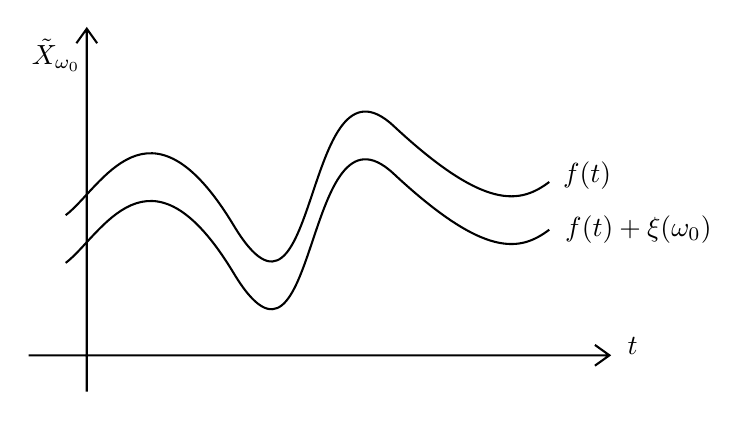
\begin{tikzpicture}[x=0.75pt,y=0.75pt,yscale=-1,xscale=1]
%uncomment if require: \path (0,184); %set diagram left start at 0, and has height of 184

%Shape: Axis 2D [id:dp08158054854684882] 
\draw  (0,158.35) -- (279.8,158.35)(27.98,1) -- (27.98,175.84) (272.8,153.35) -- (279.8,158.35) -- (272.8,163.35) (22.98,8) -- (27.98,1) -- (32.98,8)  ;
%Curve Lines [id:da7411522804130599] 
\draw    (17.8,90.84) .. controls (34.83,78.06) and (57.8,27.84) .. (98.8,95.84) .. controls (139.8,163.84) and (131.8,6.84) .. (175.8,47.84) .. controls (219.8,88.84) and (236.73,85.39) .. (250.8,74.84) ;
%Curve Lines [id:da8151172960839677] 
\draw    (17.8,113.84) .. controls (34.83,101.06) and (57.8,50.84) .. (98.8,118.84) .. controls (139.8,186.84) and (131.8,29.84) .. (175.8,70.84) .. controls (219.8,111.84) and (236.73,108.39) .. (250.8,97.84) ;

% Text Node
\draw (256,63.4) node [anchor=north west][inner sep=0.75pt]    {$f( t)$};
% Text Node
\draw (257,89.4) node [anchor=north west][inner sep=0.75pt]    {$f( t) +\xi ( \omega _{0})$};
% Text Node
\draw (287,148.4) node [anchor=north west][inner sep=0.75pt]    {$t$};
% Text Node
\draw (0,4.4) node [anchor=north west][inner sep=0.75pt]    {$\tilde{X}_{\omega _{0}}$};


\end{tikzpicture}

\end{example}
\begin{example}
Пусть $\displaystyle \{\xi _{n} ,\ n\in \mathbb{N}\}$ -- независимые случайные векторы из $\displaystyle \mathbb{R}^{m}$. Обозначим $\displaystyle S_{0} =0,\ S_{n} =\xi _{1} +\ \dotsc \ +\xi _{n} ,\ n\geqslant 1$. Случайный процесс $\displaystyle \{S_{n} ,\ n\in \mathbb{Z}_{+}\}$ является процессом с дискретным временем и называется \textit{случайным блужданием}.
\end{example}
\begin{example}
Пусть $\displaystyle \{\xi _{n} ,\ n\in \mathbb{N}\}$ -- невырожденные независимые одинаково распределенные случайнные величины, причем $\displaystyle \xi _{n} \geqslant 0\ \forall n\in \mathbb{N}$. Определим $\displaystyle S_{0} =0,\ S_{n} =\xi _{1} +\ \dotsc \ +\xi _{n}$. Тогда случайный процесс $\displaystyle X=( X_{t} ,\ t\geqslant 0)$, где $\displaystyle X_{0} =0,\ X_{t} =\sup _{n\in \mathbb{N}}\{n:\ S_{n} \leqslant t\} ,\ t\neq 0$ называется \textit{процессом восстановления}, построенным по случайным величинам $\displaystyle \{\xi _{n} ,\ n\in \mathbb{N}\}$. Траектория случайного процесса имеет вид




\tikzset{every picture/.style={line width=0.75pt}} %set default line width to 0.75pt        

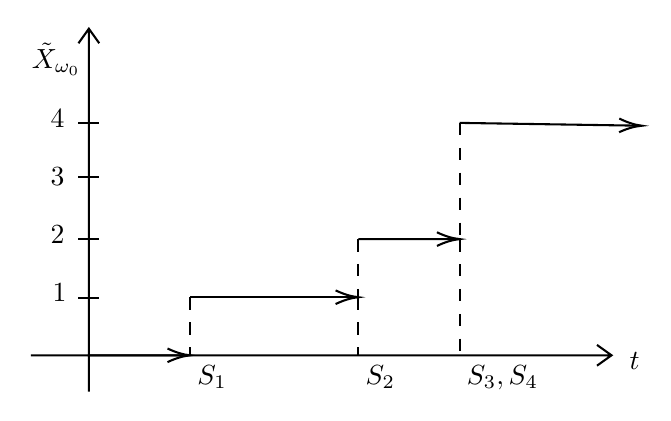
\begin{tikzpicture}[x=0.75pt,y=0.75pt,yscale=-1,xscale=1]
%uncomment if require: \path (0,184); %set diagram left start at 0, and has height of 184

%Shape: Axis 2D [id:dp8475000076862125] 
\draw  (0,158.35) -- (279.8,158.35)(27.98,1) -- (27.98,175.84) (272.8,153.35) -- (279.8,158.35) -- (272.8,163.35) (22.98,8) -- (27.98,1) -- (32.98,8)  ;
%Straight Lines [id:da26579493128629306] 
\draw    (27.98,158.35) -- (74.8,158.36) ;
\draw [shift={(76.8,158.36)}, rotate = 180.01] [color={rgb, 255:red, 0; green, 0; blue, 0 }  ][line width=0.75]    (10.93,-3.29) .. controls (6.95,-1.4) and (3.31,-0.3) .. (0,0) .. controls (3.31,0.3) and (6.95,1.4) .. (10.93,3.29)   ;
%Straight Lines [id:da7225196697527165] 
\draw    (76.8,130.36) -- (155.8,130.36) ;
\draw [shift={(157.8,130.36)}, rotate = 180] [color={rgb, 255:red, 0; green, 0; blue, 0 }  ][line width=0.75]    (10.93,-3.29) .. controls (6.95,-1.4) and (3.31,-0.3) .. (0,0) .. controls (3.31,0.3) and (6.95,1.4) .. (10.93,3.29)   ;
%Straight Lines [id:da010031330421115259] 
\draw    (157.8,102.36) -- (204.62,102.37) ;
\draw [shift={(206.62,102.37)}, rotate = 180.01] [color={rgb, 255:red, 0; green, 0; blue, 0 }  ][line width=0.75]    (10.93,-3.29) .. controls (6.95,-1.4) and (3.31,-0.3) .. (0,0) .. controls (3.31,0.3) and (6.95,1.4) .. (10.93,3.29)   ;
%Straight Lines [id:da5491041862612263] 
\draw    (206.62,46.37) -- (292.44,47.71) ;
\draw [shift={(294.44,47.74)}, rotate = 180.89] [color={rgb, 255:red, 0; green, 0; blue, 0 }  ][line width=0.75]    (10.93,-3.29) .. controls (6.95,-1.4) and (3.31,-0.3) .. (0,0) .. controls (3.31,0.3) and (6.95,1.4) .. (10.93,3.29)   ;
%Straight Lines [id:da20069256658075307] 
\draw  [dash pattern={on 4.5pt off 4.5pt}]  (76.8,130.36) -- (76.8,158.36) ;
%Straight Lines [id:da5922937776947677] 
\draw  [dash pattern={on 4.5pt off 4.5pt}]  (157.8,102.36) -- (157.8,130.36) ;
%Straight Lines [id:da9919186838924294] 
\draw  [dash pattern={on 4.5pt off 4.5pt}]  (206.62,46.37) -- (206.62,102.37) ;
%Straight Lines [id:da20620239310075394] 
\draw  [dash pattern={on 4.5pt off 4.5pt}]  (157.8,130.36) -- (157.8,158.36) ;
%Straight Lines [id:da9671890296282326] 
\draw  [dash pattern={on 4.5pt off 4.5pt}]  (206.62,102.37) -- (206.62,158.37) ;
%Straight Lines [id:da11994584273740183] 
\draw    (22.8,130.56) -- (32.8,130.56) ;
%Straight Lines [id:da9533302824156062] 
\draw    (22.75,102.34) -- (32.75,102.34) ;
%Straight Lines [id:da08575322044041878] 
\draw    (22.75,72.34) -- (32.75,72.34) ;
%Straight Lines [id:da04909413941241758] 
\draw    (22.75,46.34) -- (32.75,46.34) ;

% Text Node
\draw (287,155.4) node [anchor=north west][inner sep=0.75pt]    {$t$};
% Text Node
\draw (-1,6.4) node [anchor=north west][inner sep=0.75pt]    {$\tilde{X}_{\omega _{0}}$};
% Text Node
\draw (78.8,161.76) node [anchor=north west][inner sep=0.75pt]    {$S_{1}$};
% Text Node
\draw (159.8,161.76) node [anchor=north west][inner sep=0.75pt]    {$S_{2}$};
% Text Node
\draw (208.62,161.77) node [anchor=north west][inner sep=0.75pt]    {$S_{3} ,S_{4}$};
% Text Node
\draw (9,122.4) node [anchor=north west][inner sep=0.75pt]    {$1$};
% Text Node
\draw (8,94.4) node [anchor=north west][inner sep=0.75pt]    {$2$};
% Text Node
\draw (8,66.4) node [anchor=north west][inner sep=0.75pt]    {$3$};
% Text Node
\draw (8,38.4) node [anchor=north west][inner sep=0.75pt]    {$4$};


\end{tikzpicture}

\end{example}
\begin{proposition}
Процесс восстановления конечен почти наверное.
\end{proposition}
\begin{proof}
Пусть $\displaystyle E\xi _{i} =a< \infty $. Зафиксируем $\displaystyle t$ и рассмотрим событие $\displaystyle \{X_{t} =+\infty \}$:
\begin{equation*}
\{X_{t} =+\infty \} =\{\forall n:\ S_{n} \leqslant t\} =\bigcap _{n=1}^{\infty }\{S_{n} \leqslant t\} .
\end{equation*}
Заметим, что $\displaystyle \{S_{n+1} \leqslant t\} \subset \{S_{n} \leqslant t\}$, то в силу непрерывности меры
\begin{equation*}
P( X_{t} =+\infty ) =\lim _{n\rightarrow \infty } P( S_{n} \leqslant t) =\lim _{n\rightarrow \infty } P\left(\dfrac{S_{n}}{n} \leqslant \dfrac{t}{n}\right) .
\end{equation*}
Так как $\displaystyle t$ фиксирован, то при достаточно большом $\displaystyle n$ выполнится $\displaystyle \dfrac{t}{n} \leqslant \dfrac{a}{2}$. Тогда
\begin{equation*}
\lim _{n\rightarrow \infty } P\left(\dfrac{S_{n}}{n} \leqslant \dfrac{t}{n}\right) \leqslant \lim _{n\rightarrow \infty } P\left(\dfrac{S_{n}}{n} \leqslant \dfrac{a}{2}\right) .
\end{equation*}
В силу ЗБЧ $\displaystyle \dfrac{S_{n}}{n}\xrightarrow{P} a\Rightarrow \dfrac{S_{n}}{n}\xrightarrow{d} a\Rightarrow \lim _{n\rightarrow \infty } P\left(\dfrac{S_{n}}{n} \leqslant \dfrac{a}{2}\right) =P\left( a\leqslant \dfrac{a}{2}\right) =0$. Значит, $\displaystyle \forall t\hookrightarrow P( X_{t} =+\infty ) =0$. В силу неубывания по $\displaystyle t$ функции $\displaystyle X_{t}$ при фиксированном $\displaystyle \omega $ получаем
\begin{equation*}
P( \exists t:\ X_{t} =+\infty ) \leqslant P( \exists n\in \mathbb{N} :\ X_{n} =+\infty ) =0.
\end{equation*}
Если $\displaystyle E\xi _{i} =\infty $, то определим $\displaystyle \tilde{\xi }_{i} =\min( \xi _{i} ,\ 1)$. Тогда $\displaystyle \tilde{S}_{n} =\tilde{\xi }_{1} +\ \dotsc \ +\tilde{\xi }_{n} \leqslant S_{n}$. По уже доказанному $\displaystyle 0=\lim _{n\rightarrow \infty } P\left(\tilde{S}_{n} \leqslant t\right) \geqslant \lim _{n\rightarrow \infty } P( S_{n} \leqslant t)$.
\end{proof}
\begin{example}
Пусть $\displaystyle \{\xi _{n} ,\ n\in \mathbb{N}\}$ -- невырожденные независимые одинаково распределенные случайные величины, причем $\displaystyle \xi _{i} \geqslant 0$. Пусть $\displaystyle ( X_{t} ,\ t\geqslant 0)$ -- процесс восстановления по $\displaystyle \{\xi _{n} ,\ n\in \mathbb{N}\}$. Также, пусть $\displaystyle \{\eta _{n} ,\ n\in \mathbb{N}\}$ -- независимые одинаково распределенные случайные величины, причем $\displaystyle \eta _{i} \geqslant 0$ и независимы с $\displaystyle \{\xi _{n}\}$, $\displaystyle y_{0} ,\ c >0$ -- числа. Тогда \textit{моделью страхования Спарре Андерсена} называется процесс $\displaystyle ( Y_{t} ,\ t\geqslant 0)$, где $\displaystyle Y_{t} =y_{0} +ct-\sum _{k=1}^{X_{t}} \eta _{k}$. Траектория случайного процесса имеет следующий вид


\tikzset{every picture/.style={line width=0.75pt}} %set default line width to 0.75pt        

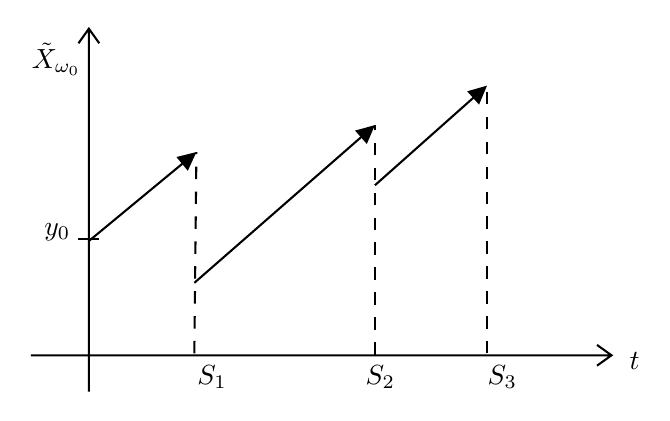
\begin{tikzpicture}[x=0.75pt,y=0.75pt,yscale=-1,xscale=1]
%uncomment if require: \path (0,184); %set diagram left start at 0, and has height of 184

%Shape: Axis 2D [id:dp8676016483616931] 
\draw  (0,158.35) -- (279.8,158.35)(27.98,1) -- (27.98,175.84) (272.8,153.35) -- (279.8,158.35) -- (272.8,163.35) (22.98,8) -- (27.98,1) -- (32.98,8)  ;
%Straight Lines [id:da622585146975575] 
\draw    (22.75,102.34) -- (32.75,102.34) ;
%Straight Lines [id:da5065640055255607] 
\draw    (27.8,103.44) -- (77.49,62.35) ;
\draw [shift={(79.8,60.44)}, rotate = 140.41] [fill={rgb, 255:red, 0; green, 0; blue, 0 }  ][line width=0.08]  [draw opacity=0] (8.93,-4.29) -- (0,0) -- (8.93,4.29) -- cycle    ;
%Straight Lines [id:da11645758297969766] 
\draw  [dash pattern={on 4.5pt off 4.5pt}]  (78.8,157.44) -- (79.8,60.44) ;
%Straight Lines [id:da8844301878317509] 
\draw    (78.8,123.44) -- (163.54,49.41) ;
\draw [shift={(165.8,47.44)}, rotate = 138.86] [fill={rgb, 255:red, 0; green, 0; blue, 0 }  ][line width=0.08]  [draw opacity=0] (8.93,-4.29) -- (0,0) -- (8.93,4.29) -- cycle    ;
%Straight Lines [id:da6782670307997067] 
\draw  [dash pattern={on 4.5pt off 4.5pt}]  (165.8,158) -- (165.8,47.44) ;
%Straight Lines [id:da07903047278333397] 
\draw    (165.8,76.44) -- (217.56,30.43) ;
\draw [shift={(219.8,28.44)}, rotate = 138.37] [fill={rgb, 255:red, 0; green, 0; blue, 0 }  ][line width=0.08]  [draw opacity=0] (8.93,-4.29) -- (0,0) -- (8.93,4.29) -- cycle    ;
%Straight Lines [id:da6248635445604189] 
\draw  [dash pattern={on 4.5pt off 4.5pt}]  (219.8,157.44) -- (219.8,28.44) ;

% Text Node
\draw (287,155.4) node [anchor=north west][inner sep=0.75pt]    {$t$};
% Text Node
\draw (-1,6.4) node [anchor=north west][inner sep=0.75pt]    {$\tilde{X}_{\omega _{0}}$};
% Text Node
\draw (78.8,161.76) node [anchor=north west][inner sep=0.75pt]    {$S_{1}$};
% Text Node
\draw (159.8,161.76) node [anchor=north west][inner sep=0.75pt]    {$S_{2}$};
% Text Node
\draw (218.62,161.77) node [anchor=north west][inner sep=0.75pt]    {$S_{3}$};
% Text Node
\draw (5,93.4) node [anchor=north west][inner sep=0.75pt]    {$y_{0}$};


\end{tikzpicture}
\end{example}
\begin{note}
Параметры в модели страхования Спарре Андерсена имеют следующий смысл: $\displaystyle y_{0}$ -- начальный капитал, $\displaystyle c$ -- скорость поступления страховых взносов, $\displaystyle \xi _{n}$ -- время между $\displaystyle ( n-1)$-ой и $\displaystyle n$-ой выплатами, $\displaystyle \eta _{n}$ -- размер $\displaystyle n$-ой выплаты, $\displaystyle X_{t}$ -- число выплат к моменту времени $\displaystyle t$.
\end{note}